\documentclass[Física - Práctica.root.tex]{subfiles}

\newcommand{\gravity}[1][per-mode=fraction]{\SI[#1]{9,8}{\meter\per\second\squared}}

\begin{document}

\section{Unidad 6}
\subsection{Parte 1}
\begin{enumerate}
  \item Un hombre arrastra hacia arriba un baúl por la rampa de un camión de mudanzas. La rampa está inclinada \ang{20,0} y el hombre tira hacia arriba con una fuerza cuya dirección forma un ángulo de \ang{30,0} con la rampa, como muestra la figura.

        \begin{center}
          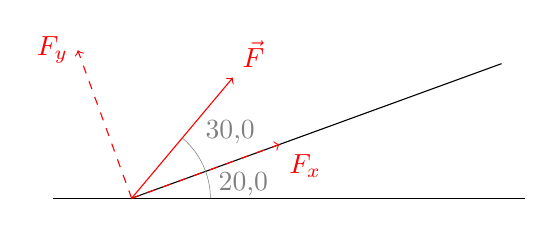
\begin{tikzpicture}
            \draw (-1,0) -- ++(6,0);
            \draw (0,0) -- ++(20:5);
            \draw[help lines] (0,0) ++(0:1) arc (0:20:1) node[pos=.5, right]{\ang{20,0}};
            \draw[help lines] (0,0) ++(20:1) arc (20:50:1) node[pos=.5, above right]{\ang{30,0}};
            \draw[red, ->] (0,0) -- ++(50:2) node[above right]{$\vec{F}$};
            \draw[red, dashed, ->] (0,0) -- ++(20:2) node[below right]{$F_x$};
            \draw[red, dashed, ->] (0,0) -- ++(110:2) node[left]{$F_y$};
          \end{tikzpicture}
        \end{center}

        \begin{enumerate}
          \item ¿Qué fuerza se necesita para que la componente $F_x$ paralela a la rampa sea de \SI{60,0}{\newton}?

                \[F_x=\vec{F}\cos{\theta}\]
                \[\SI{60,0}{\newton}=\vec{F}\cos{\ang{30,0}}\]
                \[\vec{F}=\frac{\SI{60,0}{\newton}}{\cos{\ang{30,0}}}=\boxed{\SI{69,3}{\newton}}\]

          \item ¿Qué magnitud tendrá entonces la componente $F_y$ perpendicular a la rampa?

                \[F_y=\vec{F}\sin{\theta}=\SI{69,3}{\newton}\cdot\sin{\ang{30,0}}=\boxed{\SI{34,5}{\newton}}\]
        \end{enumerate}

  \item Un hombre sale de comprar del supermercado y se dirige a guardar la mercadería comprada en su auto, para llegar al estacionamiento empuja el carrito cargado de mercadería con una fuerza resultante de \SI{600}{\newton}, como consecuencia adquiere una aceleración de \SI{1,50}{\meter\per\second\squared}.

        \begin{enumerate}
          \item Calcular la masa del carrito con la mercadería.

                \[F=ma\]
                \[\SI{600}{\newton}=m\cdot\SI{1,50}{\meter\per\second\squared}\]
                \[m=\frac{\SI{600}{\newton}}{\SI{1,50}{\meter\per\second\squared}}=\boxed{\SI{400}{\kilogram}}\]

          \item Si se descargó la tercera parte de la mercadería del carrito y se vuelve a aplicar la misma fuerza resultante ¿Cuál es ahora la aceleración del carrito?

                \[F=ma\]
                \[\SI{600}{\newton}=\frac{2}{3}\cdot\SI{400}{\kilogram}\cdot a\]
                \[a=\frac{\SI{600}{\newton}}{\frac{2}{3}\cdot\SI{400}{\kilogram}}=\boxed{\SI{2,25}{\meter\per\second\squared}}\]
        \end{enumerate}

  \item Dos cajas, una de \SI{4,00}{\kg} de masa y la otra con una masa de \SI{6,00}{\kg} descansan en la superficie sin fricción de un estanque congelado, unidas por una cuerda delgada como muestra la figura. Una persona con zapatos de golf (los cuales le dan tracción sobre el hielo) aplica un tirón horizontal $F$ a la caja de \SI{6,00}{\kg} y le imparte una aceleración de \SI{2,50}{\meter\per\second\squared}.

        \begin{center}
          \begin{tikzpicture}
            \draw (-1,0) -- ++(10,0);
            \draw (0,0) rectangle ++(2,3) node[pos=.5]{\SI{4,00}{\kg}};
            \draw (1,3) node[above]{$\beta$};
            \draw (2,1.5) -- ++(2,0);
            \draw[red, <->] (2,1.7) -- ++(2,0) node[pos=.5, above]{$T$};
            \draw (4,0) rectangle ++(2,3) node[pos=.5]{\SI{6,00}{\kg}};
            \draw (5,3) node[above]{$\alpha$};
            \draw[red, ->] (6,1.5) -- ++(2,0) node[right]{$F$};
            \draw[green, ->] (6,2) -- ++(2,0) node[right]{\SI{2,50}{\meter\per\second\squared}};
          \end{tikzpicture}
        \end{center}

        \begin{enumerate}
          \item ¿Qué aceleración tiene la caja de \SI{4,00}{\kg}?

                \[a_\beta=a_\alpha=\boxed{\SI{2,50}{\meter\per\second\squared}}\]

          \item Dibujé un diagrama de cuerpo libre para la caja de \SI{4,00}{\kg} y calcule la $T$ensión en la cuerda que une a las dos cajas.

                \begin{center}
                  \begin{tikzpicture}
                    \draw (-.5,-.5) rectangle ++(1,1);
                    \draw[red, ->] (0,0) -- ++(0,-1) node[below]{$g$};
                    \draw[red, ->] (0,0) -- ++(0,1) node[above]{$-g$};
                    \draw[red, ->] (0,0) -- ++(1,0) node[right]{$T$};
                  \end{tikzpicture}
                \end{center}

                \[F=ma\]
                \[T=\SI{4,00}{\kg}\cdot\SI{2,50}{\meter\per\second\squared}=\boxed{\SI{10,0}{\newton}}\]

          \item Calcular la magnitud de la fuerza ejercida por la persona.

                \[F=ma\]
                \[F=(\SI{4,00}{\kg}+\SI{6,00}{\kg})\cdot\SI{2,50}{\meter\per\second\squared}=\boxed{\SI{25,0}{\newton}}\]
        \end{enumerate}

  \item Dos carretones, $A$ y $B$, cuyas masas son \SI{80,0}{\kg} y \SI{120}{\kg} respectivamente, se encuentran uno junto al otro, como muestra la figura, apoyados sobre un piso horizontal que no presenta rozamiento. Sobre el carretón $A$ se aplica una fuerza horizontal de \SI{300}{\newton}.

        \begin{center}
          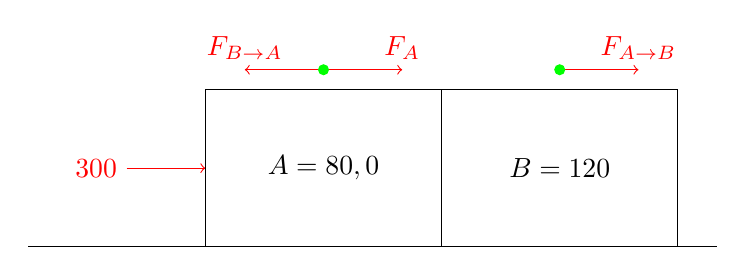
\begin{tikzpicture}
            \draw (-2.25,0) -- (6.5,0);
            \draw[red, ->] (-1,1) node[left]{\SI{300}{\newton}} -- ++(1,0);
            \draw (0,0) rectangle ++(3,2) node[pos=.5]{$A=\SI{80,0}{\kg}$};
            \coordinate (a) at (1.5,2.25);
            \draw[red, ->] (a) -- ++(1,0)  node[above]{$F_A$};
            \draw[red, ->] (a) -- ++(-1,0) node[above]{$F_{B\to A}$};
            \fill[green] (a) circle(2pt);

            \draw (3,0) rectangle ++(3,2) node[pos=.5]{$B=\SI{120}{\kg}$};
            \coordinate (b) at (4.5,2.25);
            \draw[red, ->] (b) -- ++(1,0)  node[above]{$F_{A\to B}$};
            \fill[green] (b) circle(2pt);
          \end{tikzpicture}
        \end{center}

        \begin{enumerate}
          \item Calcular la magnitud de la fuerza aplicada entre ambos carretones.

                \[F_B=\SI{300}{\newton}\cdot\frac{\SI{120}{\kg}}{\SI{80,0}{\kg}+\SI{120}{\kg}}=\SI{180}{\newton}\]

          \item Calcular ahora la magnitud de la fuerza aplicada entre ambos carretones si la fuerza horizontal de \SI{300}{\newton} se hubiese aplicado de derecha a izquierda sobre el carretón $B$.

                \[F_A=\SI{300}{\newton}\cdot\frac{\SI{80,0}{\kg}}{\SI{80,0}{\kg}+\SI{120}{\kg}}=\SI{120}{\newton}\]
        \end{enumerate}

  \item  Los dos bloques están unidos por una cuerda gruesa uniforme de peso despreciable. Se aplica una fuerza de \SI{200}{\newton} hacia arriba como se ilustra en la figura.

        \begin{center}
          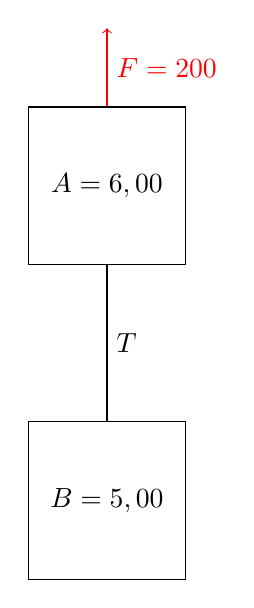
\begin{tikzpicture}
            \draw[red, ->] (0,1) -- ++(0,1) node[pos=.5, right]{$F=\SI{200}{\newton}$};
            \draw (-1,-1) rectangle ++(2,2) node[pos=.5]{$A=\SI{6,00}{\kg}$};
            \draw (0,-1) -- ++(0,-2) node[pos=.5, right]{$T$};
            \draw (-1,-5) rectangle ++(2,2) node[pos=.5]{$B=\SI{5,00}{\kg}$};
          \end{tikzpicture}
        \end{center}

        \begin{enumerate}
          \item Realice en proporción los diagramas de cuerpo libre para el bloque de \SI{6,00}{\kg} y el de \SI{5,00}{\kg}.

                \begin{multicols}{2}
                  \begin{center}
                    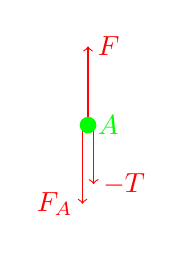
\begin{tikzpicture}
                      \draw[red, ->] (-2pt,0) -- ++(0,-1) node[left]{$F_A$};
                      \draw[red, ->] (2pt,0) -- ++(0,-.75) node[right]{$-T$};
                      \draw[red, ->] (0,0) -- ++(0,1) node[right]{$F$};
                      \fill[green] circle(3pt) node[right]{$A$};
                    \end{tikzpicture}
                  \end{center}
                  \begin{center}
                    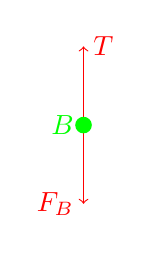
\begin{tikzpicture}
                      \draw[red, ->] (0,0) -- ++(0,-1) node[left]{$F_B$};
                      \draw[red, ->] (0,0) -- ++(0,1) node[right]{$T$};
                      \fill[green] circle(3pt) node[left]{$B$};
                    \end{tikzpicture}
                  \end{center}
                \end{multicols}

          \item ¿Que aceleración tiene el sistema?

                \[F_A=m_Ag=\SI{6,00}{\kg}\cdot\SI{-9,80}{\meter\per\second\squared}=\SI{-58,8}{\newton}\]
                \[F_B=\SI{5,00}{\kg}\cdot\SI{-9,80}{\meter\per\second\squared}=\SI{-49,0}{\newton}\]

                \[
                  a
                  =\frac{\Sigma F}{\Sigma m}
                  =\frac{F+F_A+F_B+\cancel{T-T}}{m_A+m_B}
                  =\frac{\SI{200}{\newton}-\SI{58,8}{\newton}-\SI{49,0}{\newton}}{\SI{6,00}{\kg}+\SI{5,00}{\kg}}
                  =\boxed{\SI{8,38}{\meter\per\second\squared}}
                \]

          \item ¿Cuánto es la magnitud de la Tensión en la cuerda?

                \[F=ma\]
                \[T+F_B=m_Ba\]
                \[T-\SI{49,0}{\newton}=\SI{5,00}{\kg}\cdot\SI{8,38}{\meter\per\second\squared}\]
                \[T=\boxed{\SI{90,9}{\newton}}\]
        \end{enumerate}

  \item El gráfico muestra la fuerza resultante aplicada a un móvil que, partiendo del reposo, se mueve en la dirección $x$ sin rozamiento. ¿Cuál de las siguientes afirmaciones es verdadera? Argumente por qué las demás son erróneas.

        \begin{multicols}{3}
          \begin{center}
            \begin{tikzpicture}
              \draw (0,0) -- ++(4,0) node[right]{$x$};
              \draw[->] (0,0) -- ++(0,2) node[left]{$F$};
              \draw[red] (0,0) -- (2,2) -- (4,0);
              \draw[help lines, dashed] (2,0) -- (2,2);
              \draw[help lines, dashed] (2,0) -- ++(0,2);
              \draw (0,0) node[below]{$0$};
              \draw (2,0) node[below]{$A$};
              \draw (4,0) node[below]{$B$};
            \end{tikzpicture}
          \end{center}

          \begin{center}
            \begin{tikzpicture}
              \draw (0,0) -- ++(4,0) node[right]{$x$};
              \draw[->] (0,0) -- ++(0,2) node[left]{$a$};
              \draw[red] (0,0) -- (2,2) -- (4,0);
              \draw[help lines, dashed] (2,0) -- (2,2);
              \draw[help lines, dashed] (2,0) -- ++(0,2);
              \draw (0,0) node[below]{$0$};
              \draw (2,0) node[below]{$A$};
              \draw (4,0) node[below]{$B$};
            \end{tikzpicture}
          \end{center}

          \begin{center}
            \begin{tikzpicture}
              \draw (0,0) -- ++(4,0) node[right]{$x$};
              \draw[->] (0,0) -- ++(0,2) node[left]{$V$};
              \draw[red] (0,0) parabola (2,1) parabola bend (4,2) (4,2);
              \draw[help lines, dashed] (2,0) -- ++(0,2);
              \draw (0,0) node[below]{$0$};
              \draw (2,0) node[below]{$A$};
              \draw (4,0) node[below]{$B$};
            \end{tikzpicture}
          \end{center}
        \end{multicols}

        \begin{enumerate}
          \item La velocidad es máxima en la posición A.

                Falso.
          \item Desde 0 hasta B la aceleración es constante.

                Falso.
          \item Entre A y B la velocidad disminuye.

                Falso.
          \item En A la aceleración es máxima.

                Verdadero.
          \item En A el móvil cambia el sentido de movimiento.

                Falso.
        \end{enumerate}

  \item El tambor de un lavarropas tiene \SI{40}{\cm} de diámetro y puede centrifugar las prendas a una velocidad de \SI{1200}{rpm} (revoluciones por minuto). ¿A qué fuerza se verá sometida una prenda mojada de \SI{2}{\kg}?
\end{enumerate}

\subsection{Parte 2}
\begin{enumerate}
  \item Un niño se encuentra jugando con un palo y un disco de hockey en un lago congelado de
        Canadá, cuando el niño golpea al disco con su bastón, al cual le proporciona una rapidez
        inicial de \SI{20,0}{\meter\per\second}. El disco permanece en el hielo disminuyendo su velocidad
        constantemente hasta detenerse a una distancia \SI{120}{\meter}.
        \begin{enumerate}
          \item ¿Cuál es la aceleración con que el disco se detiene?

                \[
                  \begin{cases}
                    X_f = X_i + V_it + \frac{1}{2}at^2
                    \\
                    V_f = V_i + at
                  \end{cases}
                \]\[
                  \begin{cases}
                    \SI{120}{\meter} = \SI{20}{\meter\per\second}t + \frac{1}{2}at^2
                    \\
                    \SI{0}{\meter\per\second} = \SI{20}{\meter\per\second} + at
                  \end{cases}
                \]\[
                  \begin{cases}
                    \SI{120}{\meter} = t(\SI{20}{\meter\per\second} + \frac{1}{2}at)
                    \\
                    -\SI{20}{\meter\per\second} = at
                  \end{cases}
                \]

                \[ \SI{120}{\meter} = t(\SI{20}{\meter\per\second} + \frac{1}{2}(-\SI{20}{\meter\per\second})) \]
                \[ \SI{120}{\meter} = t(\SI{20}{\meter\per\second} - \frac{1}{2}\SI{20}{\meter\per\second}) \]
                \[ \SI{120}{\meter} = t(\SI{20}{\meter\per\second} - \SI{10}{\meter\per\second}) \]
                \[ \SI{120}{\meter} = \SI{10}{\meter\per\second}t \]
                \[ \frac{\SI{120}{\meter}}{\SI{10}{\meter\per\second}} = t \]
                \[ t = \SI{12}{\second} \]
                \\
                \[ \SI{0}{\meter\per\second} = \SI{20}{\meter\per\second} + at \]
                \[ \SI{0}{\meter\per\second} = \SI{20}{\meter\per\second} + a\SI{12}{\second} \]
                \[ -\SI{20}{\meter\per\second} = a\SI{12}{\second} \]
                \[ a
                  = \frac{-\SI{20}{\meter\per\second}}{\SI{12}{\second}}
                  = 1,\overline{6}\si[per-mode=fraction]{\meter\per\second\squared}
                  \approx \boxed{\SI[per-mode=fraction]{1,7}{\meter\per\second\squared}}
                \]

          \item Determine el coeficiente de fricción entre el disco y el hielo.

                \[ |f_k| = \mu_k|n| \]
                \[ m\cdot \SI[per-mode=fraction]{1,7}{\meter\per\second\squared} = \mu_k\cdot gm \]
                \[ \SI[per-mode=fraction]{1,7}{\meter\per\second\squared} = \mu_k\cdot g \]
                \[ g = \gravity \]
                \[ \SI[per-mode=fraction]{1,7}{\meter\per\second\squared} = \mu_k\cdot\gravity \]
                \[ \mu_k = \frac{
                    \SI{1,7}{\meter\per\second\squared}
                  }{
                    \gravity[per-mode=reciprocal]
                  } \]
                \[ \boxed{\mu_k = \num{0,170}} \]

        \end{enumerate}

  \item
        \begin{multicols}{2}
          El coeficiente de fricción estática entre la caja de masa de \SI{3,00}{\kilogram}
          y el plano inclinado de \ang{35,0} es de \num{0,300}. ¿Cuál es la fuerza
          mínima $\vec{F}$ perpendicular al plano que debe ser aplicada a la caja
          para evitar que ésta deslice por la pendiente?
          \begin{center}
            \begin{tikzpicture}
              \coordinate (F) at (35:5);
              \draw[thin, draw=gray] (0,0) -- (1,0) arc [start angle=0, end angle=35, radius=1] node[right,pos=0.5]{$\alpha = \ang{35,0}$} -- cycle;
              \draw (0,0) -- (F);
              \draw (0,0) -- (F |- 0,0);
              \begin{scope}[rotate=35]
                \coordinate (B) at (2,0);
                \draw (B) rectangle +(1,1);
                \draw[fvec] (B) ++(0.5,2) -- +(0,-1) node[above left, pos=0]{$\vec{F}$};
                \draw[fvec] (B) ++(0.5,0.5) -- ++(-125:1) node[right, pos=0.1]{$\vec{g}$};
                \fill[red] (B) ++(0.5,0.5) circle[radius=0.05];
              \end{scope}
            \end{tikzpicture}
          \end{center}
        \end{multicols}
        \begin{center}
          \begin{tikzpicture} % Diagrama de cuerpo libre
            \draw[black] (-1,-1) rectangle +(2,2);
            \begin{scope}[fvec, near end] % Dibujar vectores
              \draw circle[radius=0.05];
              \draw (0,0) -- (0,2.5) node[right]{$\vec{n}$};
              \draw (0,0) -- (0,-2) node[right]{$\vec{F}$};
              \draw (0,0) -- (-125:1 |- 0,-2) node[left]{$\vec{F}_g$};
              \draw (0,0) -- ++(2,0) node[above]{$\vec{f}_s$};
            \end{scope}
          \end{tikzpicture}
          \begin{tikzpicture} % Diagrama del vector F_g
            \draw[help lines] (0,-0.5) arc[start angle=-90, end angle=-125, radius=0.5] node[below,pos=0.5]{$\alpha$};
            \begin{scope}[fvec] % Dibujar vectores
              \draw (0,0) -- node[right]{$\vec{F}_{g\bot}$} (0,-3) node(R){}; % Perpendicular
              \draw (0,0) -- node[left]{$\vec{F}_g$} (-125:3 |- R) node(G){}; % Gravedad
              \draw (R) -- node[below right]{$\vec{F}_{g\parallel}$} (G) node(B){}; % Paralelo
            \end{scope}
          \end{tikzpicture}
        \end{center}

        \begin{multicols}{2}
          \begin{center}
            \[ \sin\alpha = \frac{F_{g\parallel}}{F_g} \]
            \[ \sin\alpha = \frac{F_{g\parallel}}{m\cdot g} \]
            \[ \sin\ang{35,0} = \frac{F_{g\parallel}}{\SI{3,00}{\kilogram}\gravity[per-mode=reciprocal]} \]
            \[ \sin\ang{35,0} = \frac{F_{g\parallel}}{\SI{29,4}{\newton}} \]
            \[ \SI{29,4}{\newton}\sin\ang{35,0} = F_{g\parallel} \]
            \[ F_{g\parallel} = \SI{16,7}{\newton} \]
          \end{center}
          \begin{center}
            \[ \cos\alpha = \frac{F_{g\bot}}{F_g} \]
            \[ \cos\alpha = \frac{F_{g\bot}}{m\cdot g} \]
            \[ \cos\ang{35,0} = \frac{F_{g\bot}}{\SI{3,00}{\kilogram}\gravity[per-mode=reciprocal]} \]
            \[ \cos\ang{35,0} = \frac{F_{g\bot}}{\SI{29,4}{\newton}} \]
            \[ \SI{29,4}{\newton}\cos\ang{35,0} = F_{g\bot} \]
            \[ F_{g\bot} = \SI{24,1}{\newton} \]
          \end{center}
        \end{multicols}
        \begin{center}
          \[ n = F_{g\bot} + F \]
          \[ f_s = n\cdot\mu_s \]
          \[ \sum F_x = 0 \]
          \[ \sum F_x = F_{g\parallel} - f_s = 0 \]
          \[ F_{g\parallel} - n\cdot\mu_s = 0 \]
          \[ F_{g\parallel} - (F_{g\bot} + F)\cdot\mu_s = 0 \]
          \[ \SI{16,7}{\newton} - (\SI{24,1}{\newton} - F)\cdot\num{0,300} = 0 \]
          \[ \SI{16,7}{\newton} - \SI{7,23}{\newton} - F\cdot\num{0,300} = 0 \]
          \[ \SI{9,47}{\newton} = F\cdot\num{0,300} \]
          \[ \frac{\SI{9,47}{\newton}}{\num{0,300}} = F \]
          \[ \boxed{F = \SI{31,6}{\newton}} \]
        \end{center}

  \item
        \begin{multicols}{2}
          Una mujer en el aeropuerto mueve su maleta de \SI{20,0}{\kilogram} a una
          velocidad constante tirando de la correa con una fuerza de \SI{35,0}{\newton} con
          una dirección $\theta$ determinada como muestra la figura, la fuerza de
          fricción entre la maleta y el piso es de \SI{20,0}{\newton}.
          \begin{center}
            \begin{tikzpicture}
              \draw[black] (-1,-1) rectangle +(2,2);
              \begin{scope}[help lines]
                \draw (0,0) -- (2,0 -| 30:2);
                \draw (0.5,0) arc [start angle=0, end angle=30, radius=0.5] node[right,pos=0.5]{$\alpha$};
              \end{scope}
              \begin{scope}[fvec] % Vectores
                \draw circle[radius=0.05];
                \draw (0,0) -- (30:2) node[above]{$\vec{F}$};
                \draw (0,0) -- (0,-2) node[right,near end]{$\vec{g}$};
                \draw (0,0) -- (-2,0) node[above]{$\vec{f}_s$};
              \end{scope}
            \end{tikzpicture}
          \end{center}
        \end{multicols}
        \begin{enumerate}
          \item ¿Qué ángulo forma la correa con respecto a la horizontal cuando la mujer jala de ella?
                \begin{center}
                  \[ a = 0 \Rightarrow \sum F_x = 0 \]
                  \[ \sum F_x = \vec{F}_x - f_s = 0 \]
                  \[ \vec{F}_x = f_s \]
                  \[ \vec{F}_x = F\cdot cos(\alpha) \]
                  \[ f_s = F\cdot cos(\alpha) \]
                  \[ \SI{20,0}{\newton} = \SI{35}{\newton}\cdot cos(\alpha)\]
                  \[ cos(\alpha) = \frac{\SI{20,0}{\newton}}{\SI{35,0}{\newton}} \]
                  \[ \alpha = arcos(\frac{4}{7}) \]
                  \[ \boxed{\alpha = \ang{55,2}} \]
                \end{center}
          \item ¿Cuál es la fuerza normal que ejerce la tierra sobre la maleta?
                \begin{center}
                  \[ \sum F_y = 0 \]
                  \[ \sum F_y = F_g - \vec{F}_y - n = 0 \]
                  \[ F_g - \vec{F}_y = n \]
                  \[ m\cdot g - Fsin(\alpha) = n \]
                  \[ \SI{20,0}{\kilogram}\cdot \gravity - \SI{35,5}{\newton}sin(\ang{55,2}) = n \]
                  \[ \boxed{n = \SI{167}{\newton}} \]
                \end{center}
        \end{enumerate}

  \item
        \begin{multicols}{2}
          La caja A de la figura tiene una masa de \SI{4,00}{\kilogram} y el
          bloque B, de \SI{12,0}{\kilogram}. El coeficiente de fricción cinética
          entre el bloque B y la mesa es de \num{0,25}.
          \begin{center}
            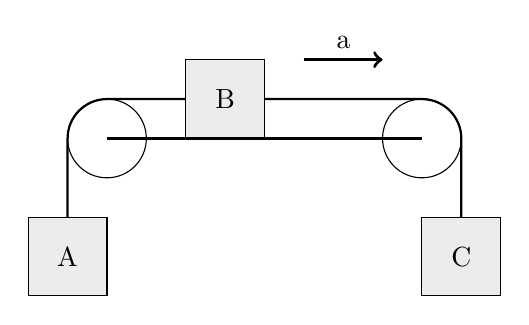
\begin{tikzpicture}
              %\draw[dashed,very thin,gray] (-5,-5) grid (5,5);
              \draw[thin] (-1.5,0) arc[start angle=0,end angle=360,radius=0.5]; % Rueda izq.
              \draw[thin] (2.5,0) arc[start angle=0,end angle=360,radius=0.5]; % Rueda der.
              \draw[thick] (-2.5,-1) -- ++(0,1) arc[start angle=180, end angle=90,radius=0.5] -- ++(1,0) node(A){}; % Cuerda izq.
              \draw[thick] (A) ++(1,0) -- ++(2,0) arc[start angle=90, end angle=0,radius=0.5] -- +(0,-1); % Cuerda der.
              \draw[very thick,->] (A) ++(1.5,0.5) -- node[above]{a} ++(1,0); % Fuerza `a`
              \begin{scope}[fill=gray!15] % Cajas
                \filldraw (-3,-2) rectangle +(1,1) node[pos=0.5]{A};
                \filldraw (-1,0) rectangle +(1,1) node[pos=0.5]{B};
                \filldraw (2,-2) rectangle +(1,1) node[pos=0.5]{C};
              \end{scope};
              \draw[very thick] (-2,0) -- (2,0); % Piso
            \end{tikzpicture}
          \end{center}
        \end{multicols}
        \begin{enumerate}
          \item ¿Qué masa tiene el bloque C si el bloque B se mueve de izquierda a derecha con una aceleración de \SI[per-mode=fraction]{2}{\meter\per\second\squared}?
          \item ¿Qué tensión hay en cada cuerda cuando el bloque B tiene esa aceleración?
        \end{enumerate}

  \item Un objeto experimenta un MAS (movimiento armónico simple) con periodo de \SI{1,200}{\second} y
        amplitud de \SI{0,600}{\meter}. En el tiempo inicial el objeto está en $x = 0$ y se mueve en la dirección
        negativa $x$. \\
        ¿Qué tan lejos se encuentra el objeto de la posición de equilibrio cuando transcurrió un
        tiempo de \SI{0,480}{\second}?
        \begin{center}
          \[ T = \SI{1,200}{\second} \]
          \[ A = \SI{-0,600}{\meter} \]
          \[ \omega = \frac{\Delta\theta}{\Delta t} \]
          \[ \omega = \frac{\SI{2\pi}{\radian}}{\SI{1,200}{\second}} \]
          \[ \omega = \SI[per-mode=symbol]{1,667}{\radian\per\second} \]
          \[ \sin\ang{0} = 0 \]
          \[ A\sin(\omega t) \]
          \[ (\SI{-0,600}{\meter})\cdot\sin(t\cdot\SI[per-mode=symbol]{1,667}{\radian\per\second}) \]
          \[
            (\SI{-0,600}{\meter}) \cdot \sin( \SI{0,480}{\second} \cdot \SI[per-mode=symbol]{1,667}{\radian\per\second} )
            = \SI{-0,353}{\meter}
          \]
          \[ \boxed{
              | \SI{-0,353}{\meter} | = \SI{0,353}{\meter}
            } \]
        \end{center}

  \item Un cuerpo de masa desconocida se une a un resorte ideal con una constante de \SI{120}{N/m}.
        Se observa que vibra con una frecuencia de \SI{6,00}{\hertz}.
        \begin{enumerate}
          \item Calcule el periodo del movimiento.
                \[ \SI{6,00}{\hertz} = \frac{\SI{1}{\second}}{6} \approx \boxed{\SI{0,167}{\second}} \]
          \item Calcule la frecuencia angular.
                \[ T = \SI{0,167}{\second} \]
                \[ \omega = \frac{\Delta\theta}{\Delta T} \]
                \[ \omega = \frac{\SI{2\pi}{\radian}}{\SI{0,167}{\second}} \]
                \[ \boxed{
                    \omega = \SI[per-mode=symbol]{37,7}{\radian\per\second}}
                \]
          \item Calcule la masa del cuerpo.
                \[ \omega^2 = \frac{k}{m} \]
                \[ k = \SI{120}{N/m} \]
                \[ \omega = \SI{37,7}{\per\second} \]
                \[ (\SI{37,7}{\per\second})^2 = \frac{\SI{120}{N/m}}{m} \]
                \[ \SI{1421,29}{\per\second\squared} = \frac{\SI{120}{\kilo\gram\cancel\meter\per\second\squared\per\cancel\meter}}{m} \]
                \[ m = \frac{\SI{120}{\kilo\gram\per\cancel\second\squared}}{\SI{1421,29}{\cancel\per\second\squared}} \]
                \[ \boxed{ m = \SI{0,0844}{\kilo\gram} } \]
        \end{enumerate}


  \item Una caja de herramientas de \SI{45,0}{\kilogram} descansa sobre un piso horizontal. Usted le aplica
        una fuerza horizontal cada vez mayor, y observa que la caja empieza a moverse cuando la
        fuerza excede los \SI{313}{\newton}. Después, debe reducir la fuerza a \SI{208}{\newton} para mantener la caja de
        herramientas a una velocidad constante de \SI[per-mode=symbol]{25,0}{\centi\meter\per\second}.
        \begin{enumerate}
          \item ¿Cuáles son los coeficientes de fricción estático y cinético entre la caja y el piso?
                \begin{center}
                  \begin{tikzpicture}
                    \draw[black] (-0.5,-0.5) rectangle ++(1,1);
                    \filldraw[red] (0,0) circle[radius=0.05];
                    \begin{scope}[fvec, near end]
                      \draw (0,0) -- node[above]{$\vec{F}_1$}(1.5,0);
                      \draw (0,0) -- node[above]{$\vec{f_s}$}(-1,0);
                      \draw (0,0) -- node[right]{$\vec{n}$}(0,1.3);
                      \draw (0,0) -- node[right]{$\vec{g}$}(0,-1.3);
                    \end{scope}
                  \end{tikzpicture}
                  \[ n = g\cdot m \]
                  \[ n = \gravity\cdot \SI{45,0}{\kilo\gram} \]
                  \[ n = \SI{441}{\newton} \]
                  \[ F_1 = n\cdot\mu_s \]
                  \[ \SI{313}{\newton} = \SI{441}{\newton}\cdot\mu_s \]
                  \[ \boxed{ \mu_s = \num{0,710} } \]
                  \begin{tikzpicture}
                    \draw[black] (-0.5,-0.5) rectangle ++(1,1);
                    \filldraw[red] (0,0) circle[radius=0.05];
                    \begin{scope}[fvec, near end]
                      \draw (0,0) -- node[above]{$\vec{F}_2$}(1.5,0);
                      \draw (0,0) -- node[above]{$\vec{f_k}$}(-1,0);
                      \draw (0,0) -- node[right]{$\vec{n}$}(0,1.3);
                      \draw (0,0) -- node[right]{$\vec{g}$}(0,-1.3);
                    \end{scope}
                  \end{tikzpicture}
                  \[ n = \SI{441}{\newton} \]
                  \[ F_2 = n\cdot\mu_k \]
                  \[ \SI{208}{\newton} = \SI{441}{\newton}\cdot\mu_k \]
                  \[ \boxed{ \mu_k = \num{0,472} } \]
                \end{center}
          \item ¿Qué fuerza debe usted ejercer para que la caja de herramientas alcance una aceleración de \SI[per-mode=symbol]{1,10}{\meter\per\second\squared}?
                \begin{center}
                  \[ F - f_k = m\cdot a \]
                  \[ F - \SI{208}{\newton} = \SI{45,0}{\kilo\gram}\cdot\SI{1,10}{\meter\per\second\squared} \]
                  \[ F = \SI{49,5}{\newton} + \SI{208}{\newton} \]
                  \[ F = \SI{258}{\newton} \]
                \end{center}
        \end{enumerate}
\end{enumerate}

\end{document}
